\subsection{执行阶段性能剖析}\label{sec:execution}

执行阶段的核心是机械臂六个 STS-3215 舵机的位置指令下发（\texttt{sync\_write}）。
为完整描述舵机链路，本节同时纳入感知阶段中物理通道完全重合的舵机位置读取
（\texttt{sync\_read}）。两者共用同一条 \texttt{/dev/ttyACM0} 半双工 TTY 总线、
相同的 SCServo 协议帧结构与 USB 串口内核路径，仅在数据包内的指令字节
（0x82 vs 0x83）和方向（写 vs 读+回包）上不同。

\subsubsection{LeRobot 执行路径软件栈}\label{sec:execution-software-stack}

图~\ref{fig:execution-callstack-software} 展示了执行阶段从
\texttt{record.py} 触发 \texttt{send\_action()} 到 \texttt{scservo\_sdk} 的
关键类关系与调用关系。

\texttt{get\_observation()} 和 \texttt{send\_action()} 分别对应
读取舵机当前位置（sync\_read）和写入目标位置（sync\_write）的两条路径，
共享 MotorsBus 层（归一化 / 符号编解码）和 Feetech 层（协议组包）。
关键数据点：Present\_Position 寄存器地址 56，写 2 字节；Goal\_Position 寄存器地址 42，写 2 字节。
读路径需等待 6 个舵机依次回包（半双工总线），写路径发完即返回，无回包。

\begin{figure}[htbp]
  \centering
  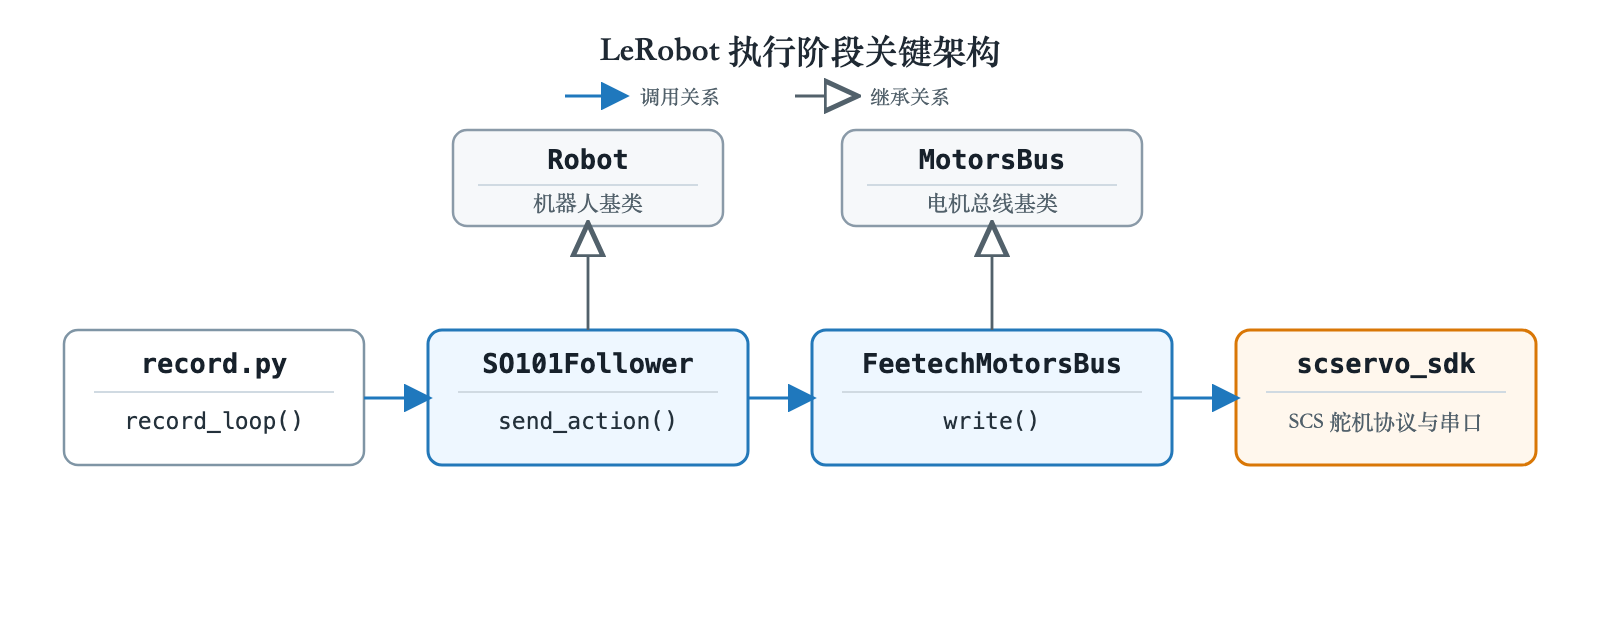
\includegraphics[width=\textwidth]{3_性能分析/image/execution_callstack_software.png}
  \caption{LeRobot 执行阶段关键类关系与调用关系}
  \label{fig:execution-callstack-software}
\end{figure}

\subsubsection{sync\_write 写链路：从电机总线到串口写入}\label{sec:sync-write-chain}

图~\ref{fig:sync-write-chain} 展示了 \texttt{send\_action()} 触发的完整写链路，
横跨五个软件层：\texttt{MotorsBus}（归一化/编码）$\to$ \texttt{GroupSyncWrite}（组包）$\to$
\texttt{GroupSyncWrite.syncWriteTxOnly()}（协议帧）$\to$ \texttt{PortHandler}（串口管理）$\to$
\texttt{ser.write()}（内核写入）。

\texttt{\_setup\_sync\_writer} 设置寄存器地址（\texttt{start\_address=42}，Goal\_Position）与数据长度（2 字节），
\texttt{addParam(id, data)} 将每个电机的目标位置序列化为 \texttt{[lo, hi]} 存入 \texttt{data\_dict[id]}；
随后 \texttt{makeParam()} 将 6 个电机数据拼成 16 字节负载，\texttt{syncWriteTxOnly()} 追加协议头与校验字节，
构造出完整的 26 字节 SYNC\_WRITE 帧（\texttt{FF FF FE 16 83 2A 02 [id lo hi] × 6 CS}），
广播 ID \texttt{0xFE} 意味着无需等待任何舵机回包；
最终 \texttt{port.writePort(pkt)} 在 \texttt{is\_using=False} 的条件下调用 \texttt{ser.write()} 将帧写入串口，
写完即返回，无 RX 阶段，随后 \texttt{clearParam()} 重置组包缓冲区。

写链路的核心特性是``发完即返回''——广播帧不要求舵机回包，Python 侧耗时约
1--3 ms，瓶颈为 USB $\to$ UART 的物理传输，而非软件开销。

\begin{figure}[htbp]
  \centering
  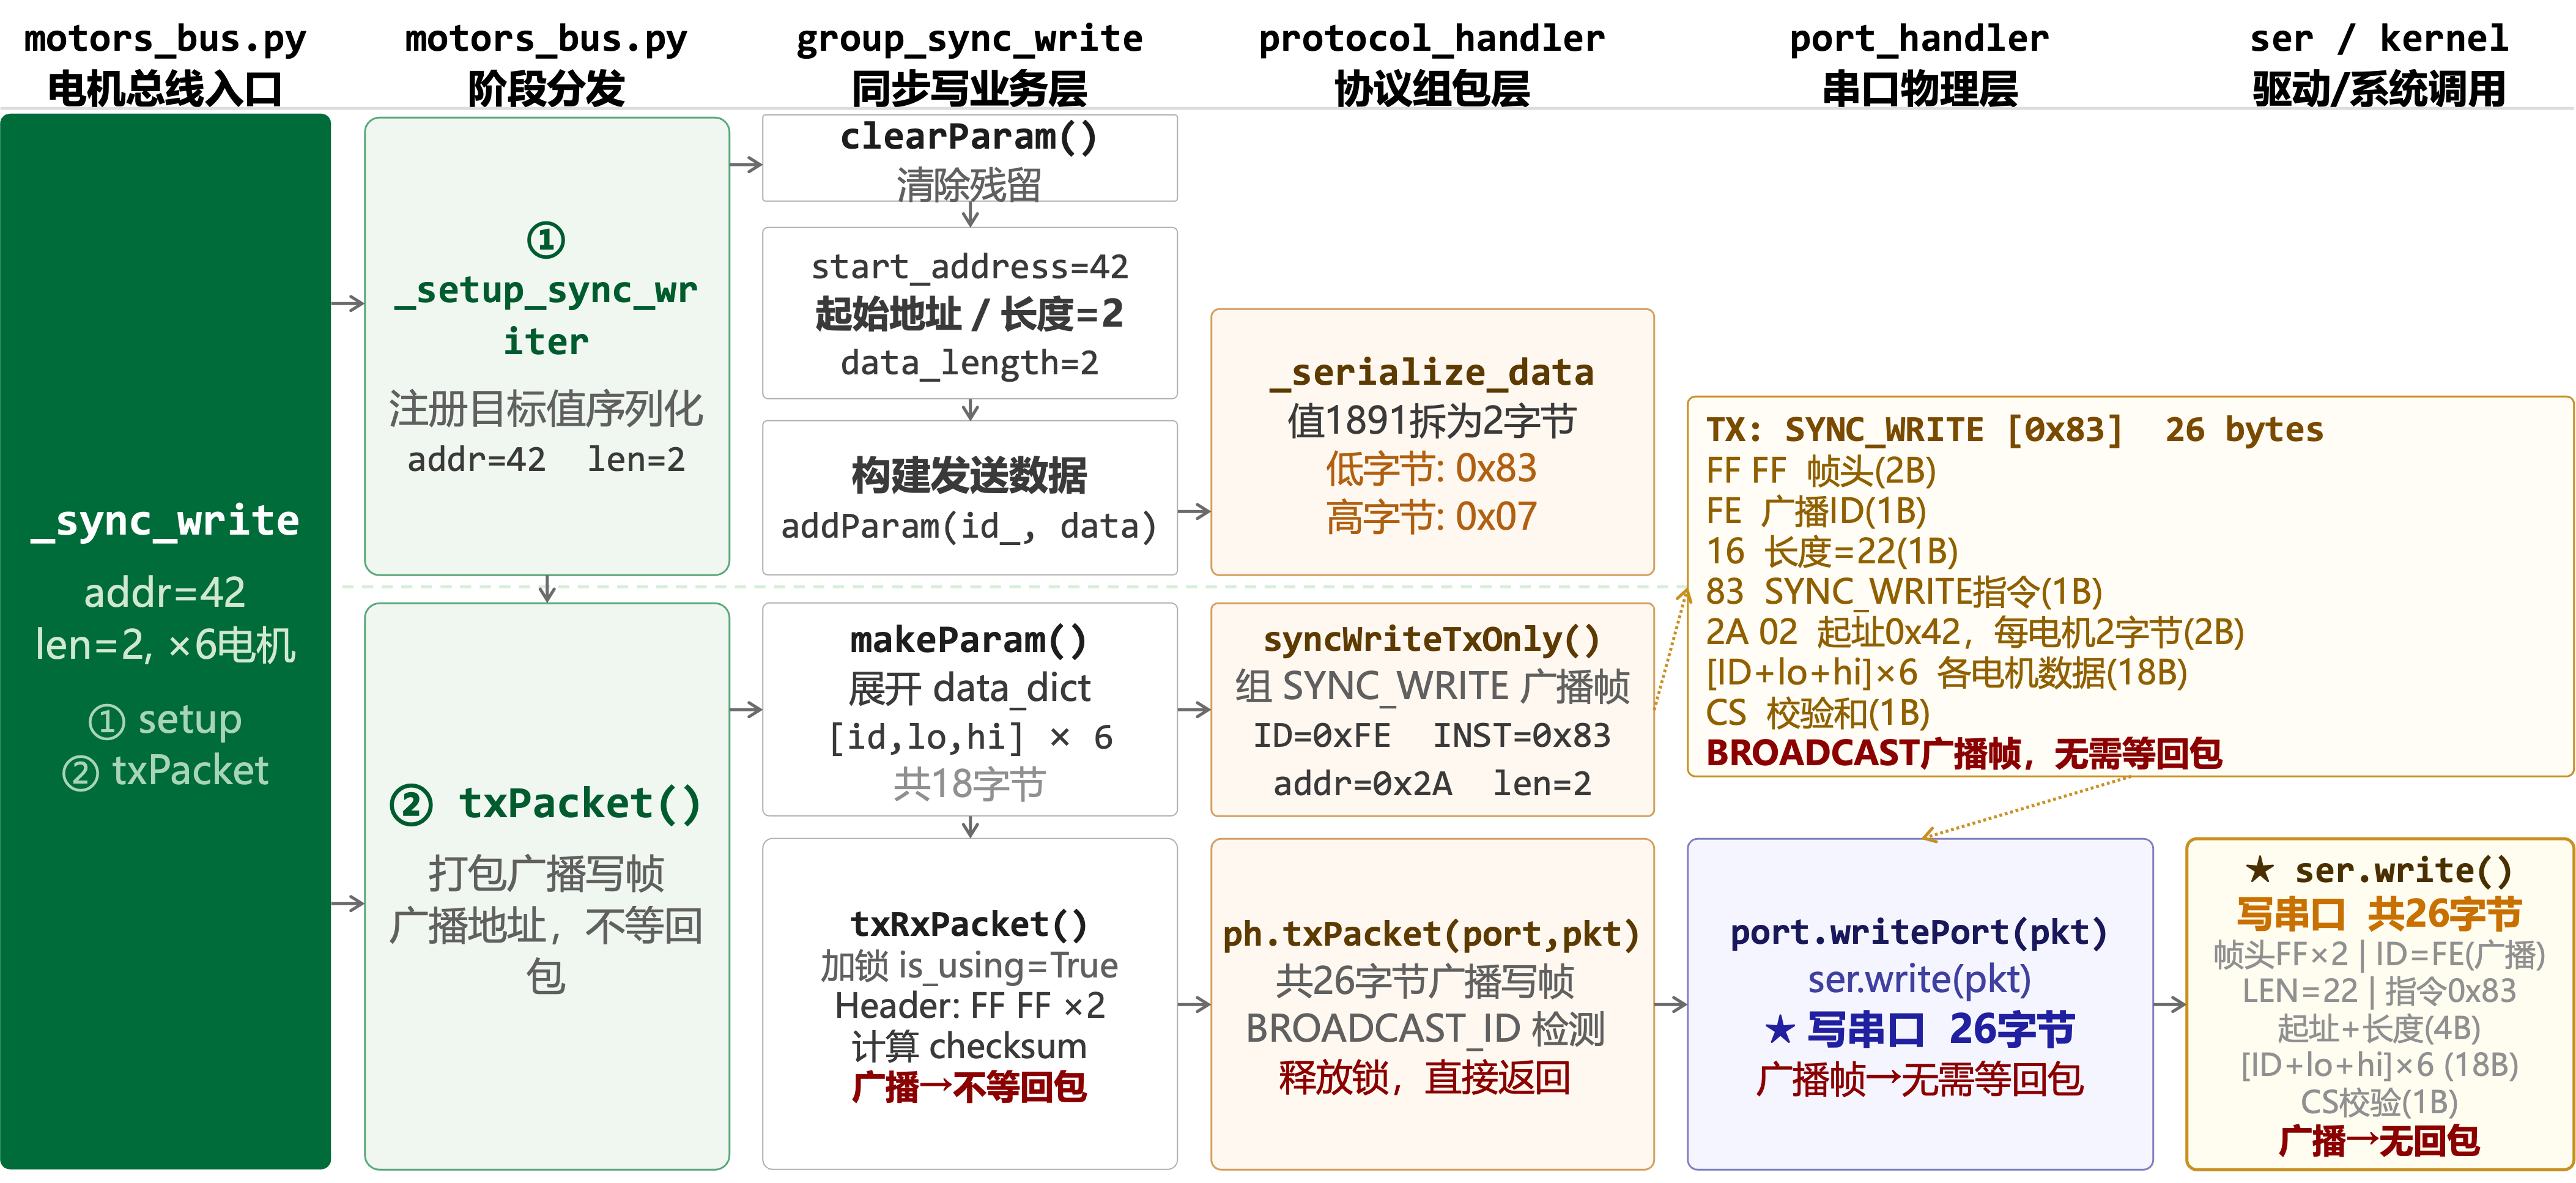
\includegraphics[width=\textwidth]{3_性能分析/image/sync_write_chain.png}
  \caption{sync\_write 写链路：motors\_bus.py $\to$ GroupSyncWrite $\to$ ProtocolHandler $\to$ PortHandler $\to$ ser.write()}
  \label{fig:sync-write-chain}
\end{figure}

\subsubsection{sync\_read 读链路：从请求帧到逐电机轮询回包}\label{sec:sync-read-chain}

图~\ref{fig:sync-read-chain} 展示了 \texttt{get\_observation()} 触发的读链路。
与写链路共享前三层软件栈，但在 \texttt{PortHandler} 层之后分叉为完整的``发送请求帧 + 逐电机轮询''双阶段。

关键数据路径如下：
\begin{enumerate}[leftmargin=2em]
  \item \textbf{请求帧发送}：\texttt{syncReadTx()} 构造 SYNC\_READ 帧
        （指令字节 \texttt{0x82}，寄存器地址 \texttt{0x38}/56，读长度 2），
        经 \texttt{ph.txPacket()} 调用 \texttt{writePort()} $\to$ \texttt{ser.write()} 写出。
        帧格式：\texttt{FF FF FE 0A 82 38 02 01 02 03 04 05 06 CS}。
  \item \textbf{逐电机回包}：\texttt{rxPacket()} 对 \texttt{data\_dict} 中每个 ID 依次调用
        \texttt{readRx(port, id, 2)}，后者调用 \texttt{ph.rxPacket(port)} $\to$ \texttt{ser.read(n)}。
        \texttt{ser.read(n)} 内部以 \texttt{while} 轮询加超时退出，等待每个电机按 ID 顺序
        在半双工总线上依次发回状态帧（\texttt{FF FF id 04 00 lo hi CS}）。
  \item \textbf{数据解析}：\texttt{getData(id, 56, 2)} 计算偏移量 \texttt{offset = 56-56 = 0}，
        取 \texttt{data[0], data[1]} 合成 16-bit 位置值（\texttt{SCS\_MAKEWORD}），
        最终返回 \texttt{\{1: 2381, …, 6: 1500\}} 形式的字典。
\end{enumerate}

读链路耗时约 1.2 ms，主要来源于 6 次串行回包等待。半双工总线在等待回包期间
不能发送任何其他指令，这是写链路无法与读链路并行化的物理根因。

\begin{figure}[htbp]
  \centering
  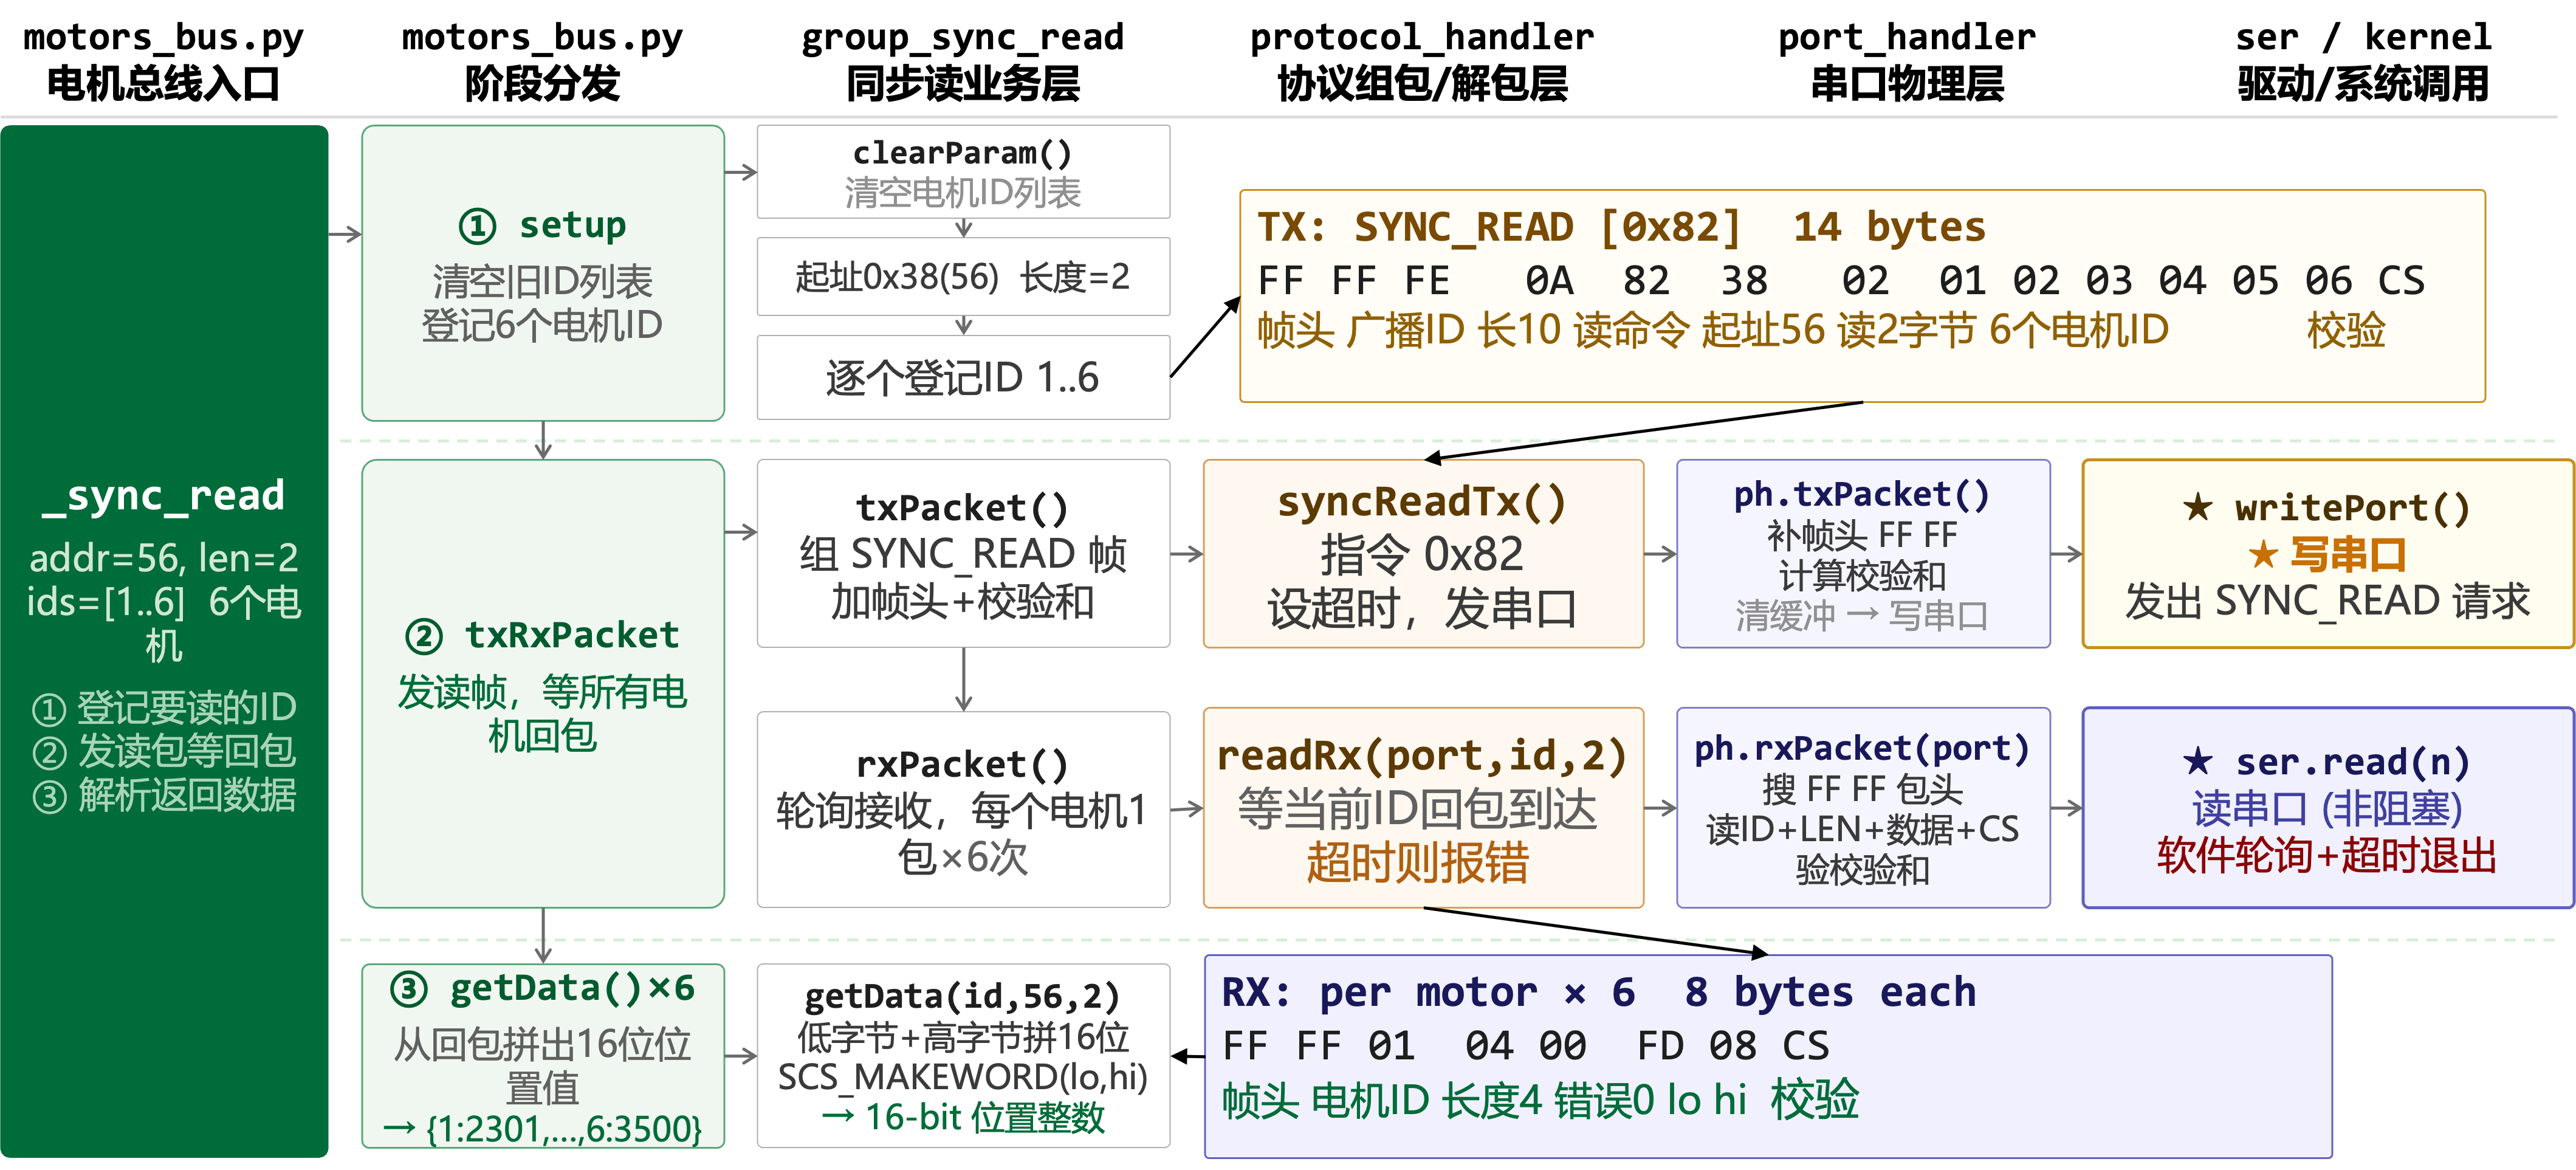
\includegraphics[width=\textwidth]{3_性能分析/image/sync_read_chain.png}
  \caption{sync\_read 读链路：motors\_bus.py $\to$ GroupSyncRead $\to$ ProtocolHandler $\to$ PortHandler $\to$ ser.read() 轮询}
  \label{fig:sync-read-chain}
\end{figure}

\textbf{关键性能结论}\label{sec:execution-conclusion}：
综合 \texttt{sync\_read} 与 \texttt{sync\_write} 两条路径可以看出，
执行阶段的主要耗时并不来自 Linux 系统调用本身。\texttt{write} 系统调用仅约
38 $\mu$s，\texttt{read} 也处于类似量级；实际观测到的 \texttt{sync\_read}
约 1.2 ms、\texttt{sync\_write} 约 1--3 ms，主要由 1 Mbps 波特率下的
SCServo 总线传输决定。具体来说，Sync Read 指令帧约 14--15 字节，
Sync Write 指令帧约 26 字节（6 ID $\times$ 4 字节位置数据，加上包头与校验），
串口物理传输时间构成耗时主体。因此，执行阶段瓶颈位于半双工舵机总线和协议物理层，
而不是 Python、SDK 封装或系统调用路径。进一步地，同一时刻总线只能容纳一个方向的传输，
若将读写简单异步并发，反而可能造成总线竞争和指令帧损坏；同时，
\texttt{send\_action()} 中 read-modify-write 的安全限幅链路依赖同步读返回的实时位置，
异步化会破坏这一控制不变量。因此，舵机读写不适合作为本文主要异步优化方向
（详见 \S\ref{sec:async-feasibility}）。
